\chapter{Fluids in Motion: Bernoulli's Principle}\index{Bernoulli's principle}\index{fluid flow}

Take a hot shower, and the curtain creeps inward and clings to your legs. Put your thumb over the
end of a garden hose, and the water shoots across the yard. Two ships sailing side by side get
pulled toward each other. A hurricane does not usually push a roof in; it lifts the roof off.

In the Buoyancy chapter, you studied fluids that sit still, where pressure depends only on depth.
This chapter is about fluids that \emph{move}. You will see one simple rule, discovered by Daniel
Bernoulli in 1738, that explains all of the puzzles above: where a fluid flows faster, its pressure
is lower.

A note on notation: the Buoyancy and Boats and Sailing chapters wrote density as $d$. From here on,
we use the Greek letter $\rho$ (rho), as physicists and engineers do, and as the Flight chapter
does. So hydrostatic pressure is $\rho gh$.

\section{Continuity: What Goes In Must Come Out}\index{continuity equation}
Water is very hard to squeeze into a smaller volume, so in a pipe or hose, every liter that flows
in one end must flow out the other. The volume passing a point each second, the \newterm{flow rate},
is the cross-sectional area times the speed: $Q = Av$. Since the flow rate is the same everywhere
along the pipe,

\begin{mdframed}[style = important, frametitle = {The Continuity Equation}]
$$A_1 v_1 = A_2 v_2$$
\end{mdframed}

Where the pipe narrows, the fluid must speed up. That is what your thumb does to a hose.

\textbf{Example}: A garden hose 2.0 cm across carries water at 1.5 m/s. You cover the end with your
thumb, leaving an opening of $0.50$ cm$^2$. How fast does the water come out?

\textbf{Solution}: The hose's area is $\pi(1.0 \text{ cm})^2 \approx 3.14$ cm$^2$. Then
$$v_2 = \frac{A_1v_1}{A_2} = \frac{3.14 \times 1.5}{0.50} \approx 9.4 \text{ m/s}$$
more than six times faster. Rivers do the same thing: where a river narrows into rapids, the water
speeds up.

\section{Bernoulli's Equation}\index{Bernoulli's equation}
Why should faster flow mean lower pressure? Think about energy. Follow a small chunk of fluid with
volume $V$ as it moves from a wide part of a pipe to a narrow part. It speeds up, so its kinetic
energy grows. Something has to do work on it to provide that energy, and the only thing pushing on
it is the surrounding fluid. So the fluid behind must push harder than the fluid in front: the pressure
must drop as the fluid speeds up.

Here is the calculation. A pressure $P$ pushing on an area $A$ makes a force $PA$; pushing the chunk a
distance $x$ does work $PAx = PV$. So the net work done on the chunk by the fluid around it is
$(P_1 - P_2)V$. By the Work and Energy chapter's work-energy idea, that work equals the chunk's gain in
kinetic plus gravitational potential energy. Its mass is $\rho V$, so
$$(P_1 - P_2)V = \tfrac{1}{2}\rho V v_2^2 - \tfrac{1}{2}\rho V v_1^2 + \rho Vg(h_2 - h_1)$$
Divide by $V$ and collect each point's terms on one side:

\begin{mdframed}[style = important, frametitle = {Bernoulli's Equation}]
$$P_1 + \tfrac{1}{2}\rho v_1^2 + \rho gh_1 = P_2 + \tfrac{1}{2}\rho v_2^2 + \rho gh_2$$
Along the flow, $P + \frac{1}{2}\rho v^2 + \rho gh$ stays the same.
\end{mdframed}

Each term is something you have met. $\rho gh$ is the hydrostatic pressure from the Buoyancy chapter.
$\frac{1}{2}\rho v^2$ is the wind pressure from the Boats and Sailing chapter, often called the
\newterm{dynamic pressure}. Bernoulli's equation says they trade off with ordinary pressure $P$: at the
same height, \textbf{where the speed goes up, the pressure goes down}. It is conservation of energy, written
for fluids.

It holds exactly for an ideal fluid: one that cannot be compressed, has no internal friction, and flows
smoothly. Water in pipes comes close. Air is compressible, but at speeds well below the speed of sound,
it behaves as if it were not, so Bernoulli's equation works well for wind and airplanes too.

\begin{figure}[H]
\centering
\begin{tikzpicture}[scale=0.85]
% pipe outline
\draw[thick] (0,0.8) -- (3,0.8) -- (4,0.35) -- (6,0.35) -- (7,0.8) -- (10,0.8);
\draw[thick] (0,-0.8) -- (3,-0.8) -- (4,-0.35) -- (6,-0.35) -- (7,-0.8) -- (10,-0.8);
\fill[sdkblue!15] (0,0.8) -- (3,0.8) -- (4,0.35) -- (6,0.35) -- (7,0.8) -- (10,0.8) -- (10,-0.8) -- (7,-0.8) -- (6,-0.35) -- (4,-0.35) -- (3,-0.8) -- (0,-0.8) -- cycle;
% vertical tubes with water columns
\fill[sdkblue!40] (1.35,0.8) rectangle (1.65,3.4);
\fill[sdkblue!40] (4.85,0.35) rectangle (5.15,2.0);
\fill[sdkblue!40] (8.35,0.8) rectangle (8.65,3.4);
\foreach \x/\b in {1.5/0.8, 5/0.35, 8.5/0.8} {
  \draw ({\x-0.15},\b) -- ({\x-0.15},3.9); \draw ({\x+0.15},\b) -- ({\x+0.15},3.9);
}
% flow arrows
\draw[-latex, thick] (0.4,0) -- (1.2,0);
\draw[-latex, thick] (4.1,0) -- (5.9,0);
\draw[-latex, thick] (8.8,0) -- (9.6,0);
\node[below, align=center, font=\small] at (1.5,-0.85) {wide:\\slow, high $P$};
\node[below, align=center, font=\small] at (5,-0.85) {narrow:\\fast, low $P$};
\node[below, align=center, font=\small] at (8.5,-0.85) {wide:\\slow, high $P$};
\end{tikzpicture}
\caption{Water flowing through a pipe that narrows (a \newterm{Venturi tube}). The water speeds up in the
narrow section (continuity), so its pressure drops there (Bernoulli). The vertical tubes show the pressure: the
water climbs less high above the narrow section.}
\label{fig:venturi}
\end{figure}

\textbf{Example}: Water flows at 2.0 m/s through a horizontal pipe that narrows from 4.0 cm$^2$ to 1.0 cm$^2$. How
much lower is the pressure in the narrow part?

\textbf{Solution}: By continuity, the water speeds up to $v_2 = \frac{4.0}{1.0}(2.0) = 8.0$ m/s. The height is the same,
so Bernoulli's equation gives
$$P_1 - P_2 = \tfrac{1}{2}\rho\left(v_2^2 - v_1^2\right) = \tfrac{1}{2}(1000)(64 - 4.0) = 30{,}000 \text{ Pa}$$
That is enough to hold up a column of water about 3 meters tall. Measuring this pressure drop is how a
\newterm{Venturi meter} measures how fast a fluid is flowing. Perfume sprayers and old car carburetors use the
same effect in reverse: fast air over the top of a thin tube lowers the pressure there, and the liquid is pushed up
the tube into the airstream.

\section{Water Out of a Tank}\index{Torricelli's law}
Punch a hole in a water tank a depth $h$ below the surface. The water at the surface is nearly still and the
water in the jet is moving fast, but both are open to the air, so both are at atmospheric pressure. The $P$ terms
cancel, and Bernoulli's equation leaves
$$\tfrac{1}{2}\rho v^2 = \rho gh \quad\Longrightarrow\quad v = \sqrt{2gh}$$
This is \newterm{Torricelli's law}: the water leaves exactly as fast as if it had fallen freely from the height of the
surface. A barrel with a hole 1.8 m below the water line squirts at $\sqrt{2(9.8)(1.8)} \approx 5.9$ m/s.

As the tank drains, $h$ shrinks, so the jet slows, and the tank drains more and more slowly. Continuity tells us how
fast the surface drops: the volume leaving through the hole each second, $a\sqrt{2gh}$, equals the tank's area $A$ times
the speed of the surface. A computer can follow this in small time steps:

\begin{minted}{python}
import math
import matplotlib.pyplot as plt

g = 9.8
tank_area = 0.5        # m^2, the tank's cross-section
hole_area = 2e-4       # m^2, a 2 cm^2 hole at the bottom
h = 1.8                # m, starting water depth
dt = 0.1               # s, one small time step

t = 0
times, depths = [0], [h]
while h > 0:
    v = math.sqrt(2 * g * h)          # Torricelli: speed of the jet
    flow = hole_area * v              # m^3 leaving each second
    h -= flow / tank_area * dt        # the surface drops (continuity)
    t += dt
    times.append(t / 60)
    depths.append(max(h, 0))

print(f"drains in {t / 60:.1f} minutes")
exact = tank_area / hole_area * math.sqrt(2 * 1.8 / g)
print(f"exact answer: {exact / 60:.1f} minutes")

plt.figure(figsize=(6, 3), dpi=200)
plt.plot(times, depths)
plt.xlabel("time (minutes)")
plt.ylabel("water depth (m)")
plt.tight_layout()
plt.savefig("draining_tank.png")
\end{minted}
\begin{verbatim}
drains in 25.2 minutes
exact answer: 25.3 minutes
\end{verbatim}

\begin{figure}[H]
\centering
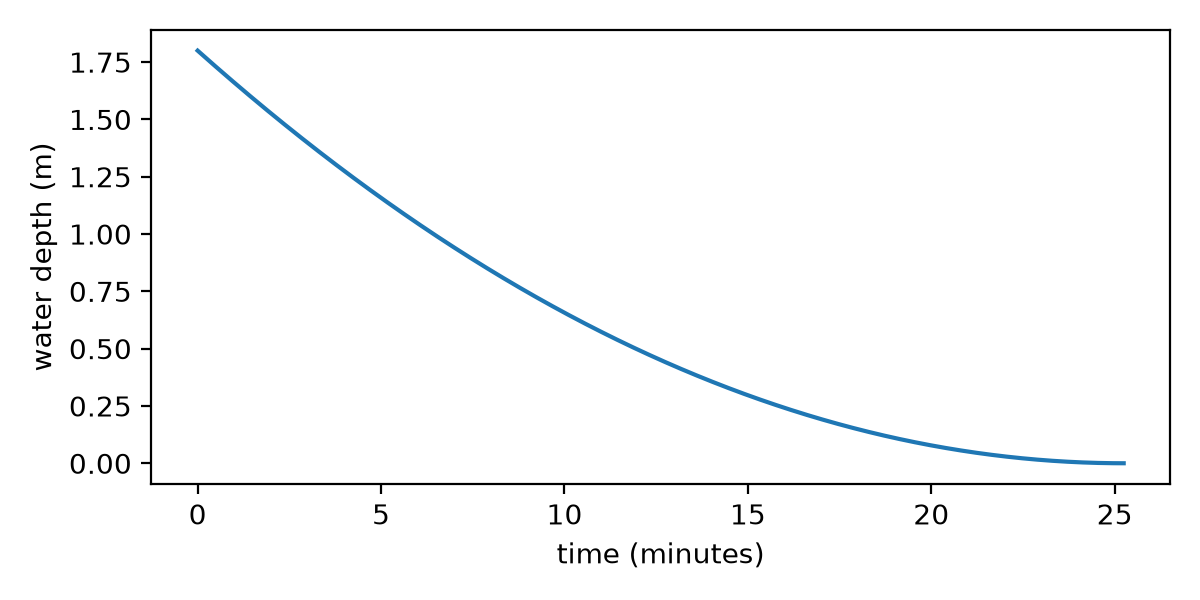
\includegraphics[width=0.7\textwidth]{draining_tank.png}
\caption{The water level falls fast at first and slowly at the end, because the jet weakens as the water gets shallower.}
\label{fig:draining-tank}
\end{figure}

\section{Explaining the Puzzles}
\textbf{The shower curtain.} The spray drags air along with it, so the air inside the shower moves faster than the still air
outside. Lower pressure inside, higher pressure outside: the curtain is pushed in.

\textbf{Passing ships.} Water rushing through the narrow channel between two ships moves faster than the water on their outer
sides. The pressure between them drops, and the water outside pushes them together. Ship captains are trained to keep their
distance for exactly this reason.

\textbf{A roof in a hurricane.} Wind at 50 m/s sweeps over a roof, while the air inside the house is still. The pressure difference
is $\frac{1}{2}\rho v^2 = \frac{1}{2}(1.2)(50^2) = 1{,}500$ Pa, which seems small. But over a 150 m$^2$ roof, it adds up to an upward force of
$225{,}000$ N, the weight of about 23 tonnes. Roofs are torn off from below, which is why hurricane building codes require
strong straps tying the roof to the walls.

\section{What About Wings?}\index{lift!and Bernoulli}
You may have heard this explanation of how wings make lift: the top of the wing is curved, so air flowing over the top has farther
to go; it must go faster to ``meet up'' with the air under the wing; faster means lower pressure; so the wing is pushed up.

The middle of that story is false. Nothing makes the two streams meet up. In wind tunnels, the air over the top of a wing actually
arrives at the back edge \emph{first}, well before the air underneath. And as the Flight chapter points out, a wing with a flat top or
an upside-down wing can still fly, if it meets the air at an angle.

Here is what really happens. A wing tilted into the air flow turns the air downward behind it. By Newton's third law, if the wing
pushes air down, the air pushes the wing up. Turning the flow also changes its speed: the air speeds up over the top and slows down
under the bottom. So Bernoulli's equation is right that the pressure is lower on top. It is just not the cause: Newton's laws and
Bernoulli's equation are two ways of describing the same flow, and both give the same lift.

\textbf{Example}: A 1,000 kg small plane has 16 m$^2$ of wing. In level flight, the lift must equal its weight. What pressure
difference does that take?

\textbf{Solution}: $\Delta P = \frac{(1000)(9.8)}{16} \approx 610$ Pa, about 0.6\% of atmospheric pressure. If the air under the wing
moves at 50 m/s, Bernoulli's equation says the air over the top needs to move only about 59 m/s:
$\frac{1}{2}(1.2)\left(59^2 - 50^2\right) \approx 610$ Pa. A small speed difference over a large area holds a plane in the sky.

The Flight chapter's lift equation, $L = \frac{1}{2}\rho v^2 S C_L$, is built on this idea: the dynamic pressure $\frac{1}{2}\rho v^2$
times the wing area, times a number $C_L$ that measures how well the wing's shape and angle turn that dynamic pressure into a
pressure difference.

\begin{Exercise}[title={A River Narrows}, label=fl_river]
A river 30 m wide and 2.0 m deep flows at 1.0 m/s. Downstream, it squeezes through a gorge 10 m wide and 3.0 m deep. How fast
does the water move in the gorge?
\end{Exercise}
\begin{Answer}[ref=fl_river]
The cross-sections are $30 \times 2.0 = 60$ m$^2$ and $10 \times 3.0 = 30$ m$^2$. By continuity,
$v_2 = \frac{60 \times 1.0}{30} = 2.0$ m/s.
\end{Answer}

\begin{Exercise}[title={Water Tower}, label=fl_tower]
The water level in a town's water tower is 20 m above a faucet. Ignoring friction in the pipes, how fast would water come out of the
open faucet? Why is the real speed lower?
\end{Exercise}
\begin{Answer}[ref=fl_tower]
By Torricelli's law, $v = \sqrt{2(9.8)(20)} \approx 19.8$ m/s. Real water slows down because of friction with the pipe walls and in
the faucet itself, which turns some of the energy into heat. Bernoulli's equation ignores that friction.
\end{Answer}

\begin{Exercise}[title={A Venturi Meter}, label=fl_venturi]
Water moves at 3.0 m/s in a horizontal pipe with a cross-section of 6.0 cm$^2$. It flows into a section with a cross-section of
2.0 cm$^2$. Find the speed in the narrow section and the drop in pressure.
\end{Exercise}
\begin{Answer}[ref=fl_venturi]
By continuity, $v_2 = \frac{6.0}{2.0}(3.0) = 9.0$ m/s. By Bernoulli,
$P_1 - P_2 = \frac{1}{2}(1000)(81 - 9.0) = 36{,}000$ Pa.
\end{Answer}

\begin{Exercise}[title={Blowing Between Two Sheets}, label=fl_paper]
Hold two sheets of paper a few centimeters apart, hanging down, and blow between them. Predict what happens, and explain why.
\end{Exercise}
\begin{Answer}[ref=fl_paper]
The sheets move \emph{together}, not apart. The fast-moving air between them has lower pressure than the still air outside, so the
outside air pushes them inward. It is the same effect that pulls passing ships together.
\end{Answer}

\begin{Exercise}[title={An Open Window?}, label=fl_window]
Some people say you should open your windows during a hurricane to ``equalize the pressure.'' Using the roof example, explain what
the pressure difference across a roof comes from, and why opening windows is not a reliable fix. (Real advice from engineers: keep
windows closed and protected.)
\end{Exercise}
\begin{Answer}[ref=fl_window]
The pressure difference comes from the fast wind over the roof (lower pressure on top, by Bernoulli's equation) compared with the
still air inside. Opening windows does not make the wind slower over the roof, and wind entering a house through an opening on the
side facing the wind can \emph{raise} the pressure inside, pushing up on the roof even harder. The roof's attachment to the walls is what
keeps it on.
\end{Answer}
